\documentclass[10pt,fleqn]{article}
\usepackage{/home/clair/Documents/mystyle}

%----------------------------------------------------------------------
% reformat section headers to be smaller \& left-aligned
\titleformat{\section}
	{\normalfont\bfseries}
	{\thesection}{1em}{}
	
\titleformat{\subsection}
	{\normalfont\bfseries}
	{\thesubsection}{1em}{}
%----------------------------------------------------------------------
% SPECIFY BIBLIOGRAPHY FILE & FIELDS TO EXCLUDE
%\addbibresource{bibfile.bib}
%\AtEveryBibitem{\clearfield{url}}
%\AtEveryBibitem{\clearfield{doi}}
%\AtEveryBibitem{\clearfield{isbn}}
%\AtEveryBibitem{\clearfield{issn}}

%======================================================================

\begin{document}

\section*{Image Processing: from .jpg to post-holes}

In order to carry out analysis on the angles and distances between the post-holes represented in a map, we first need to convert the map image into a set of points. Unfortunately, there is no standard format for the publication of archaeological plans, so it is impossible to specify a set of steps that will work for every image. However, there are a number of general steps that can be applied to any map to get a reasonably good initial separation between points and linear features, which can then be fine-tuned using more specialised functions. All of the functions referred to here have been coded as an R package and can be found at \url{https://github.com/ClairBee/AS.preprocessing}, or installed directly into R using the \texttt{install\char`_github} function in package \texttt{devtools}.

We assume (hopefully not unreasonably) that all maps will be scanned in such a way that text and other annotations, such as the legend, are more or less horizontal. Image processing prior to loading the image into R should be kept to a minimum, but cropping out figure labels and borders that are clearly external to the site plan is a useful step. Where possible, the scale key and N-S axis arrow should be kept on the scanned image, so that all measurements taken from it can be related to the site's actual scale and orientation. If this is not possible, the procedure can still be applied; evidence of regularity in the post-holes' angular and linear relationships can still be found, but without relating them to real-world measurements.

\section{Converting the map image to coordinates}

The first step is to load the .jpg file into R and convert it into a black-and-white (binary) image, using the \texttt{import.map} function. The .jpg image is loaded and converted to a raster object, which assigns a numerical colour value to the x-y coordinates of each cell in the image. At this point, with no other information available from the .jpg file, the x-coordinates are set from 0 to 1, and the y-coordinates are scaled in such a way that the aspect ratio of the image is maintained - otherwise, any perpendicular gridding in the points that we extract would be distorted. 

The raster at this point is also in full colour (although most of these colours will be shades of grey), so we need to choose a cut-point - a value between 0 and 1, with 0 being white and 1 being black, at which the intervening shades of grey are converted into one or the other. For most images, very similar outputs are obtained with thresholds anywhere from 0.1 to 0.9, however, for full-colour images a higher threshold might be necessary to avoid converting shaded areas to solid black, while for images with particularly fine or faint lines (such as the Brandon maps), a low threshold is more useful, to avoid breaking diagonal lines into smaller sections. Although this does make it more likely that small smudges and other `noise' features will be picked up, it is generally better to allow a few erroneous but randomly-distributed points such as these in the data, rather than risk wrongly identifying fragments of letters or site boundaries - which are more likely to appear in regular lines, and so to interfere with the angular analysis - as small, post-hole-type features.

Since most of the maps we have been working with are in black and white (or, at least, in very different shades of grey), the default for the function is set as 0.2, which is able to extract solid lines from the image even when they are quite finely printed, and should be perfectly adequate for most black and white images.

Once we have a strict black-and-white image, the function identifies clusters of adjacent black cells. 8-directional clumping -  including points which are diagonally adjacent on the diagonal as well as in the four cardinal directions - is used in preference to 4-directional clumping, for the same reason that a lower threshold is used for lighter images.

The result of this image processing is a list containing a raster image of the whole site plan, and a matrix containing the index number of each feature in the raster, and a label denoting how that feature is currently classified; this label is initially set to 0 (`unclassified'), but will be updated by further functions to mark features as either annotations, larger linear features of the map, part of the scale, or - finally - as post-holes.% Whenever a function is run, a new feature set is created to avoid accidentally overwriting the working data until the user chooses to do so.


\section{Identifying the scale and N-S marker}

A useful first step is to identify the scale marker and rescale the x and y coordinates of the map accordingly, so that we are working in more realistic units. The scale marker - always a long, horizontal rectangle - is generally quite straightforward to identify; the function \texttt{get.scale} searches for it by passing a focal window over the site raster, scoring highly only when it detects long horizontal lines of black cells, the largest of which is offered as a candidate scale marker. After the user provides the real length of the scale, the map's x and y coordinates are rescaled. %User confirmation is requested before any changes are made; if the user confirms that the correct object has been selected, the function requests the length that the scale represents, and will use this length to rescale the map's x and y axes appropriately.

%If the feature identified by the function is not the correct scale marker (for example, in cases where the map has a scale both in metres and in perches, and the user would prefer to work in perches), the function will offer the user the chance to select a feature by simply clicking on the map. 
The N-S marker - the style and direction of which varies widely between plans - can be manually identified from the map, using the \texttt{get.orientation} function, so that angles can later be related to the map's true orientation. 

\section{A general procedure for identifying post-hole features}

For most dig plans, the post-hole features we're interested in are represented as solid points, and are smaller than the text used to annotate the plan; the procedure below assumes that this is the case. If the post-holes are represented as hollow circles, or are larger than the text, then a different approach will be required. However, that situation generally only arises in extremely large-scale maps focussing on small areas of the larger site, which are unlikely to contain enough post-holes to make an analysis worthwhile anyway, so it is not considered further here.

It should be stressed again that the most important consideration when separating post-holes from other features is to make sure no regular features such as text or site boundaries are picked up and treated as part of the post-hole set, since this will introduce lines of points with a shared (horizontal) orientation, which is likely to have more of an adverse effect on our analysis of the angles between the post-holes than would excluding a few post-holes or including one or two accidentally-introduced random points.

\subsection{Exclude sparse features}
Positively identifying post-hole features is difficult without examining the distributions of the shapes of the features identified, which will vary from site to site depending on such factors as the resolution of the image, the scale of the map, and stylistic choices made by the printers. However, an approach that is generally extremely effective without any parameter tuning is to exclude any `sparse' features. For our purposes, a sparse feature is one where, if we were to draw the smallest possible square around the feature, and to count the number of that square's cells that the feature occupies, the ratio of occupied to empty cells would be low.

For example, consider an `ideal' post-hole object: a solid circle of black cells, with radius $r$, and covering an area of $\pi r^2$ cells. A square bounding this shape would have sides of length $2r$, and cover $4r^2$ cells, so the proportion of the cells in the square that are coloured black is $\pi/4$ (around 0.79). At the opposite end of the scale, the sparsest feature that would require a square of this size to tightly bound it is a straight line of cells, of length $2r$ and width 1, covering an area of $2r$; so the proportion of the cells that are coloured black by the line is $1/2r$, with the covered proportion growing smaller as the length of the line increases. Any cluster of only 1 or 2 cells is automatically treated as noise, so the shortest possible line is 3 pixels long, giving a maximum possible ratio for strictly linear features of 1/3; so a sensible starting threshold (and one which works well in practice), cutting midway between these two limits, is $\frac{\pi/4+1/3}{2}$, or about 0.55. 

Of course, between these two extremes there are an infinite variety of possible shapes, each covering a different proportion of its bounding square, and the exact threshold to be used can be adjusted to try to capture as much annotation as possible without including too many post-holes. For some sites - such as the Catholme plan, which has minimal annotation, with no text other than the scale marker and a boundary marked by a single solid line - this single function may be enough to filter out the post-hole features from those that hold no interest for us.

Once the sparse features have been identified, the function divides them again, into potential annotations (smaller features) and larger linear features that actually belong to the map, such as walls or roads. This distinction is fairly arbitrary and, since our focus is currently only on the post-hole data, not particularly key; it is made purely so that when using later functions that inspect each annotation sequentially, we don't have to wait for every single feature to be checked again. The function defaults to labelling any feature of more than 100 pixels as a large feature, while anything smaller is assumed to be an annotation, such as text.

% run this first since it's the quickest way to split - checking annotations only covers non-classified items, so takes much longer if we do it first

\subsection{Identify text and numbers}
Letters and numbers in the plot are often more similar in size and density to the post-holes that we are interested in than the long, linear features that we have just excluded, so further filtering is needed. Particularly in sites with a large number of text annotations, a second useful step is to look for horizontal `runs' of similarly-sized features that share a baseline, using the \texttt{remove.annotations} function. This function looks at each unclassified feature in turn, finding any objects that lie within the feature's width of its edge. Most of the labels found on the maps are numbers or upper case, and strings of such characters will share a lower edge and be of roughly the same height and width; any sequences of features that meet these criteria are therefore labelled as annotations.% As a useful (but optional) extension to this, the function stores the heights and widths of the features that it has identified as text, and will identify any other features on the map which are within 1 pixel of the modal height and width - which, assuming that all of the text annotations used on the plan share a font and point size, should pick up any last characters that do not form part of strings.

%For some sites, these two functions may be enough to identify a set of post-holes that can be worked on. However, the Genlis map - one of the main sites investigated - features text in a number of sizes, with a larger font used for the header, and slightly larger labels for the scale than are used on the main body of the map; these non-standard fonts aren't picked up by the previous function. A slightly different problem with this function arises in the Catholme map, which has no text in its body; the function needs to check around one thousand features against their neighbours, so it takes a very long time to run, for very little return. In both cases, the unclassified features consist of very small clusters of cells, most of which are post-holes, with a few letters and very short linear features remaining.

%When most of the remaining unclassified features appear to be small post-hole features, with occasional stray letters mixed in, we can use \texttt{remove.tall.features} to identify the last few tall features and mark them as annotations. The function simply obtains the heights of all remaining unclassified features and identifies outliers, using the approach applied by R when creating a boxplot: any points lying more than 1.5 times the inter-quartile range above the upper quartile are deemed to be outliers, and deemed to be non-post-hole features. This is a fairly conservative approach: only features that are unusually tall will be flagged by this function.

% Functions don't overwrite
% Once most of the remaining features are small, with perhaps only a few letters/linear features left, we can use the 'remove tall' function - in fact, in some cases it is more efficient to skip straight to this (eg. Catholme).
\subsection{`Fill in' site boundaries}
In many plans, the boundary of the excavation is marked with a broken (\texttt{-$\cdot$-}) or dashed line. Even the shortest line segments will have been identified as sparse features, but a broken line can be more problematic: in all but position, the dots resemble post-holes, but they lie on a straight line; if we accept them as post-holes, they will introduce a strong bias into our set of angles. However, we can use that fact to distinguish them from post-holes, by checking for features that are adjacent to classified annotations in any direction (rather than only to the left or right, as when checking for text). The \texttt{extend.annotations} function extends the `footprint' area of each annotation feature above, below, to the left and right of the original boundaries (rather than only horizontally, as before). The index numbers of any features that lie within the extension are recorded, and any objects that are covered by the extension of more than one annotation are also set as annotations. This means that any points on a broken line can be identified, along with decimal points and other small punctuation features that would otherwise look like post-holes among text strings.

\subsection{Extract mid-points of post-holes}
For most sites, running this simple set of steps is enough to exclude all of the non-post-hole features in the map, and the \texttt{get.postholes} function can be used to return a list of the centre-points of the remaining features (obtained by taking the mean x and y-coordinates of each feature). These centre-points define the set of points that will be used as the basis for angular analysis to identify any evidence of gridding or linearity in the data. % For particularly large sites with evidence of many separate buildings (such as Catholme or Brandon), it may prove useful to split the points into smaller clusters and analyse each one separately. %If this is the case, the best way to proceed is by using the DBscan clustering algorithm, one of few algorithms able to identify clusters of arbitrary shape rather than circular clusters. DBscan is known to be very sensitive to its parameters, but here, we have something of an advantage, in that we can use our knowledge of the site to estimate an appropriate set of parameters.


\section{Alternative approaches}
A number of further functions are available to identify any non-posthole features that aren't covered by the above procedure. If the remaining unclassified features seem to be primarily post-holes, with a few taller letters or numbers mixed in, then the function \texttt{remove.tall.features} will classify any unusually tall features as annotations, classifying them as outliers using the same approach that R uses to classify outliers in a boxplot. Features containing horizontal or vertical lines can be identified, or features classified according to the number of black cells they contain; a function also exists to manually set the class of a particular feature selected from the map. However, these latter functions require that the user provide appropriate parameters to define exactly what constitutes a post-hole-like feature and what does not. The great advantage of the functions above is that they can be applied to any site with no modifications, regardless of the site's scale or resolution, with reasonably good results. An example of the result achieved on the Genlis map using only the functions listed above is shown in Figure~\ref{fig:Genlis-result}; a few features have been retained which should have been excluded (points at the corners of the boundary, in particular, and one or two numbers in labels), but importantly, those spurious points are quite widely distributed across the map, so are only introducing noise to our data set, rather than an interfering pattern. Furthermore, any additional data cleaning that is performed - such as removing points that are outliers in terms of their nearest-neighbour distance, or clustering using an algorithm like DBscan - will most likely remove those points from the final data set.

\begin{figure}[h!]
\caption{Genlis map converted to post-holes}
\label{fig:Genlis-result}
\centering
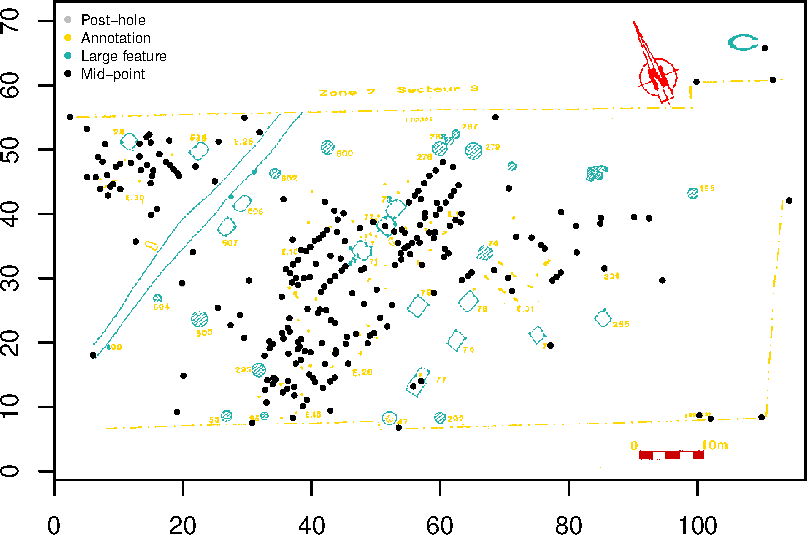
\includegraphics[scale=1]{genlis-features.pdf}
\end{figure}



\end{document}
